\documentclass[a4paper, 12pt, fleqn]{article}
\usepackage{custom}
\usepackage{titlepage}
\usepackage[bottom]{footmisc}
\usepackage{wrapfig}
\usepackage{makeidx}

%============STYLE PROPERTIES============
\setlength{\parindent}{0pt}

\graphicspath{{../}}

%============PAGE PROPERTIES=============
\newcommand{\revisiondate}{\today}
\newcommand{\documenttitle}{CM\_GlobMark} % used for title in title and subtitle pages
\newcommand{\authors}{Michael Blättler} %used for title page only
\newcommand{\subtitle}{Summary} % used for title and subtitle pages
\newcommand{\documentdesc}{Summary}
\newcommand{\ort}{Hochschule Luzern Technik \& Architektur, Horw}

%============REF-COMMANDS================
\newcommand{\secref}[1]{\hyperref[{#1}]{\autoref*{#1}}}
\providecommand{\tightlist}{\setlength{\itemsep}{0pt}\setlength{\parskip}{0pt}}

\makeindex

\begin{document}
	\begin{titlepage}
		\appendixGM
		\thispagestyle{empty}
	\end{titlepage}

	\tableofcontents

	% !TeX spellcheck = en_GB
\section{International Environments}

Helps to analyse, understand and manage the external forces enveloping the firm. It answers two basic questions:

\begin{enumerate}
	\tightlist
	\item What to analyse in the environment?
	\item How to access its relevance to the firm's strategy?
\end{enumerate}

\subsection{Outside-In and Inside-Out}
\begin{description}
	\item[Outside-In] Starts with the analysis of environmental factors and then considers all the various ways in which the firm may be affected by them.
	\item[Inside-Out] Starts with the firm’s various functions and products and then considers in each case what environmental factors may be significant.
\end{description}

\subsection{St. Gallen Management Model}
\begin{figure}[H]
	\centering
	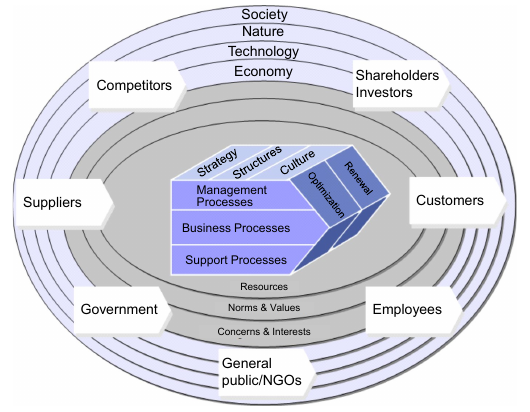
\includegraphics[width=0.8\textwidth]{figures/stgallen_mgmtModel.png}
	\caption{The new St. Gallen Management Model}
\end{figure}

\subsubsection{Environmental spheres (blue)}
Environmental spheres refer to relevant reference spaces in the environment of the company. The company interacts with the elements of these systems, which is why they are very closely analyzed for trends and changes. \textbf{Society} is the most comprehensive of these spheres. However, \textbf{technology}, \textbf{economics} and \textbf{nature} are also important.

\subsubsection{Stakeholders (white ``arrows'')}
Stakeholders refer to all groups and individuals who are somehow affected by the value or damage created by companies. The value added for these stakeholders is the purpose of a company. Claims of different parties, however, are necessarily conflict-laden, which is why the company has to find rules and procedures within the normative orientation process in order to prioritize.

\subsubsection{Interaction topics}
Interaction issues are the objects of the exchange relationships between stakeholders and companies around which the company communicates with its stakeholders. These are \textbf{norms and values} , \textbf{concerns and interests} as well as \textbf{resources}. Values refer to fundamental views about a worthwhile life, norms are based on them and designate explicit laws and regulations. Interests refer to immediate self-interest, while concerns are generalizable goals. These personal and cultural elements are the object-bound resources across from.

\subsubsection{Process perspective}
The most important process categories of the new St. Gallen Management Model. The St. Gallen Management Model understands an enterprise as a system of processes. Processes are routine processes that shape the everyday life of a company. In the superior mastery of these routines, especially in a short process time, is an important prerequisite for entrepreneurial success. A distinction is made between \textbf{management processes}, \textbf{business processes} and \textbf{support processes}.

\begin{description}
	\item[Management processes] Management processes encompass all basic tasks related to the design, direction (steering) and development of purpose-oriented socio-technical organizations.
	\item[Business processes] Business processes embody the core activities of a business, which are geared directly to customer value. They include the customer processes (brand management processes, customer acquisition processes and customer loyalty processes), the service creation processes and the performance innovation processes.
	\item[Support proccesses] This is where in-house services for an effective completion of business processes are accomplished. These include, for example, processes of educational work (learning processes) and personnel work (continuing education programs).
\end{description}

\subsubsection{Ordering moments}
Everyday life, which takes place in the form of processes, calls for a coherent orientation and meaning. These functions fulfill the order moments. They arise explicitly and implicitly from everyday life and structure this in turn. So there is a circular connection between processes and order moments. The sub-areas are \textbf{strategy}, \textbf{structures} and \textbf{culture}. 

\begin{description}
	\item[Strategy] As mentioned earlier, the strategy is based on long-term decisions that build competitive advantage. The strategy as a moment of order designates the content dimension ("what?"). It should provide information on the concerns, needs and forms of communication of the stakeholders , the range of services offered, the focus on added value , possible fields of cooperation and core competencies . In contrast, the strategic development process (see Management Processes) focuses on the "how?": How should the generation process be designed? How are the contents effectively communicated and communicated on different levels?
	\item[Structures] Structures are needed to define the necessary degree of division of labor, and to effectively coordinate these areas. This is done by means of organizational structures (organizational chart) and process structures (definition of which tasks have to be completed in which sequence, for example in the form of a process plan). Management can make comparatively easy changes here, since these are explicitly defined facts.
	\item[Culture] Culture refers to the implicit, enigmatic structures of a company. These include norms and values, attitudes, attitudes and reasoning patterns. The division of labor leads to a differentiation of culture within the enterprise. In culture, a key success factor of a company can be justified, because its elements are also difficult to put into words by its makers and therefore difficult to copy from other companies. For management it is a great challenge to influence the grown corporate culture, as it is anchored organically and unconsciously in the behavior and thinking of the employees in contrast to the formal organizational structure.
\end{description}

\subsubsection{Development modes}
Development modes describe the various types of development of a company. The continuous, ongoing improvement of the existing is referred to as \textbf{optimization}, while the discontinuous, only spiky creation of something completely new is represented by \textbf{renewal}.

\subsection{Factors}
\begin{figure}[H]
	\centering
	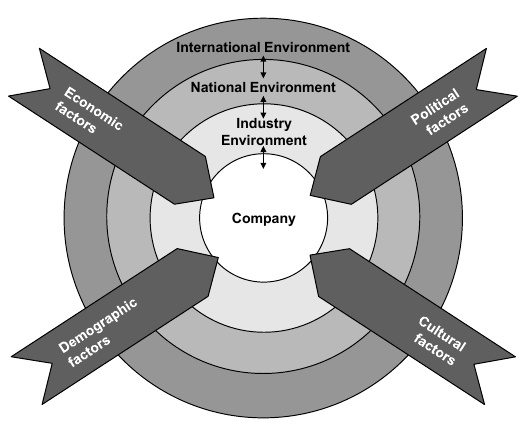
\includegraphics[width=0.6\textwidth]{figures/envAnalysisFramework.png}
	\caption{Environmental analysis framework}
\end{figure}

\subsubsection{Economic factors}

The following measurements are used as economic factors:

\begin{description}
	\item[Gross domestic product (GDP)] Gross domestic product (GDP) is a monetary measure of the market value of all the final goods and services produced in a period of time.
	\item[Openness idex] Ratio of a country's trade (exports + imports) to its GDP. $I = \frac{imports + exports}{GDP}$.
	\item[Factor movements] International factor movements are movements of labor, capital, and other factors of production between countries.
\end{description}

\paragraph{Gini index} \mbox{}\\
The Gini index measures the inequality of income distribution.\\
0 = perfect equality\\
1 = maximum inequality

\paragraph{Different types of regional integration} \mbox{}\\
\begin{figure}[H]
	\centering
	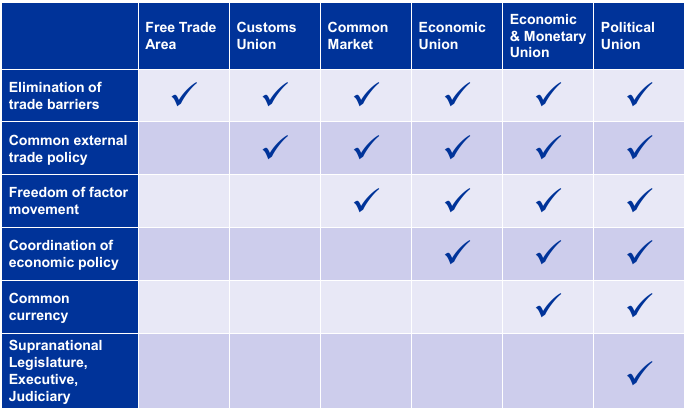
\includegraphics[width=1\textwidth]{figures/typesRegionalIntegration.png}
	\caption{Different types of regional integration}
\end{figure}

\subsubsection{Exchange rates}
Exchange rates are also part of the economic factors. Due to its importance it gets a separate subsection.

\paragraph{Terms}
\begin{description}
	\item[Nominal] The nominal exchange rate is the price of the domestic currency in terms of the foreign currency.
	\item[Real] Nominal exchange rate ($e$) adjusted by the ratio of the foreign price level ($P_f$) to the domestic price level ($P$).\\
	$RER = \frac{e\cdot P_f}{P}$
	\item[Indirect quotation or quantity quotation] 1 home currency unit = x foreign currency units\\
	1 Swiss Franc = 0.66563 Euro
	\item[Direct quotation or price quotation] 1 foreign currency unit = x home currency units\\
	1 Euro = 1.50233 Swiss Francs
	\item[Appreciation] Increase of the value of a currency relative to another currency\\
	It takes fewer Swiss Francs to purchase 1 euro
	\item[Depreciation] Decrease of the value of a currency relative to another currency\\
	It takes more Swiss Francs to purchase 1 euro
	\item[Spot exchange rate] Price that is quoted for immediate (spot) payment and delivery.
	\item[Forward exchange rate] Price that is quoted for future payment and delivery.
\end{description}


\paragraph{Currency risk}\mbox{}\\
\begin{figure}[H]
	\centering
	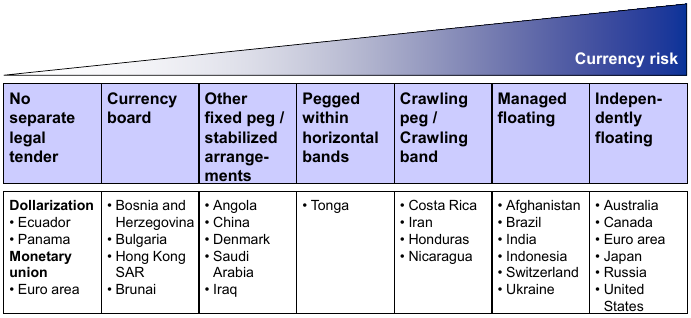
\includegraphics[width=0.9\textwidth]{figures/exchangeRegimes.png}
	\caption{Different exchange rate regimes analysed for currency risk}
\end{figure}

\begin{description}
	\item[No seperate legal tender] Basically same currency.
	\item[Currency board] Currency board is an exchange rate regime in which a country's exchange rate maintain a fixed exchange rate with a foreign currency, based on an explicit legislative commitment.
	\item[Other fixed peg/stabilized arrangements] Exchange rates are fixed due to known factors.
	\item[Pegged within horizontal bands] There is only a tiny variation around the fixed exchange rate against another currency, well within plus or minus 2\%.
	\item[Crawling peg/Crawling band] The currency steadily depreciates or appreciates at an almost constant rate against another currency. And the exchange rate follows a simple trend.
	\item[Managed floating] Managed float, also known as dirty float, involves government intervention in the market exchange rate in different forms and degrees, in an attempt to make the exchange rate change in a direction conducive to the economic development of the country, especially during an extreme appreciation or depreciation.
	\item[Independently floating] Free float, also known as clean float, signifies that a currency's value is allowed to fluctuate in response to foreign-exchange market mechanisms \textbf{without government intervention}. 
\end{description}


\subsubsection{Natural environment}
The following factors belong to the natural environment:
\begin{itemize}
	\tightlist
	\item Energy sources/consumption (Coal, Renewable, Nuclear Power, Oil)
	\item Oil reserves
	\item Metals (Copper, Aluminium, ...)
	\item Diseases (e.g. Ebola)
\end{itemize}

\subsubsection{Technological environment}
The following factors belong to the technological environment:
\begin{itemize}
	\item ICT Usage/Consumption (number of phone subscriptions, etc.)
\end{itemize}

\subsubsection{Social environment}
The following factors belong to the social environment:
\begin{itemize}
	\tightlist
	\item Population
	\item Age distribution
	\item Gender distribution
	\item Urbanization
	\item Corruption
\end{itemize}

\subsubsection{Corruption}
Corruption belongs to the social environment. Due to its importance it gets a separate subsection.
\paragraph{Terms}
\begin{description}
	\item[Definition of corruption] Any abuse of entrusted power to gain an undue (private) advantage.
	\item[Active corruption] Corrupting someone.\\
	Giving or promising to give an undue advantage in order that the opposite party should perform or refrain from performing an act, in breach of its duties.\\
	\textbf{Corrupt behaviour between private individuals.}
	\item[Passive corruption] Being corrupted oneself\\
	Requesting or receiving an undue advantage of any kind for oneself or for a third party, to perform or refrain from performing an act, in breach of ones duties.\\
	\textbf{Corrupt behaviour between private individuals and public officials}
\end{description}

\paragraph{Why combat corruption?}

\subparagraph{Economic reasons}
\begin{itemize}
	\tightlist
	\item Distorts competition
	\item Hampers transparency
	\item Leads to an inefficient distribution of resources
\end{itemize}

\subparagraph{Social and political reasons}
\begin{itemize}
	\tightlist
	\item Distorts access to public services
	\item Leads to the unlawful enrichment of individuals
	\item Undermines the rule of law and provides fertile ground for organised crime
	\item Leads to a general loss of confidence in public institutions
\end{itemize}

\subparagraph{Business reasons}
\begin{itemize}
	\tightlist
	\item Criminal liability
	\item Leads to a serious damage of the companies reputations
	\item Leads to the exclusion from public services and international projects
	\item Raises exposure to blackmailing
\end{itemize}

\paragraph{Anti corruption measures}
\begin{enumerate}
	\item Definition of operating principles
	\begin{itemize}
		\tightlist
		\item Zero tolerance policy against corruption and bribery
	\end{itemize}
	\item Situation analysis
	\begin{itemize}
		\tightlist
		\item Risk analysis (liability to corruption, existing arrangements)
		\item Country information, legal situation
	\end{itemize}
	\item Elaboration of an anti-corruption program
	\begin{itemize}
		\tightlist
		\item Field of application (all types of corruption)
		\item Internal guidelines (e.g. gifts policy, conflict of interests)
		\item Incorporation of business partners (anti-corruption clause)
		\item Sanctions
	\end{itemize}
	\item Implementation
	\begin{itemize}
		\tightlist
		\item Organizational arrangements (e.g. clear definition of respofour-eye-principle, anonymous whistleblower reporting)		
		\item Human resource management: anti-corruption employment terms, job rotation
		\item Incorporation of business partners (anti-corruption clause)
		\item Communication (internal and external)
		\item Raising awareness, anti-corruption training	
	\end{itemize}
	\item Monitoring and inspection
	\begin{itemize}
		\tightlist
		\item Internal reporting (e.g. spot checks, internal revision)	
		\item Evaluation of the measures and, if necessary, adjustments to them
	\end{itemize}
\end{enumerate}

    
    % Stichwortverzeichnis soll im Inhaltsverzeichnis auftauchen
    \addcontentsline{toc}{section}{Stichwortverzeichnis}
    
    \printindex
\end{document}